\documentclass[10pt,a4paper]{article}
\usepackage[latin1]{inputenc}
\usepackage{amsmath}
\usepackage{amsfonts}
\usepackage{amssymb}
\usepackage{color}
\usepackage{graphics}
\usepackage{graphicx}
\usepackage{hyperref}
\usepackage{biblatex}
\addbibresource{sample.bib}
\hypersetup{
	colorlinks=true,
	linkcolor=blue,
	filecolor=magenta,
	urlcolor=cyan,
}
\author{hk}
\title{test}
\begin{document}
	\color{red} First line of text\\
	\color{black}
	\textbf{Second line of text}\\
	\begin{figure}
		\centering
		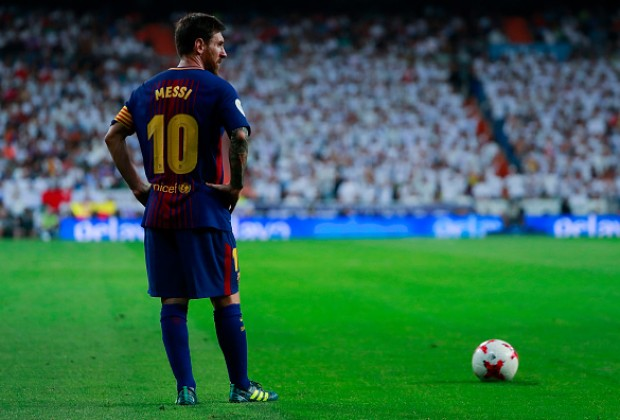
\includegraphics[width=0.9\linewidth]{messi.jpg}
	\end{figure}
	
	\begin{center}
		\begin{tabular}{|c|c|c|}
			\hline
			\textbf{cell1} & \textbf{cell2} & \textbf{cell3}\\
			\hline
			cell4 & cell5 & cell6\\
			\hline
			cell7 & cell8 & cell9\\		
			\hline
		\end{tabular}
	\end{center}
	
	$$ y^2 = (x+1)^2$$
	$$ X^{n+1}$$
	$$ x_2$$
	$$ x\;y\;z $$
	$$ \exp^2 $$
	
	\href{www.google.com}{GOOGLE}
	
	\newpage
	\bibliography{sample.bib}
	
\end{document}

